\documentclass{beamer}
\setbeamercolor{block body alerted}{bg=alerted text.fg!10}
\setbeamercolor{block title alerted}{bg=alerted text.fg!20}
\setbeamercolor{block body}{bg=structure!10}
\setbeamercolor{block title}{bg=structure!20}
\setbeamercolor{block body example}{bg=green!10}
\setbeamercolor{block title example}{bg=green!20}
\usepackage{pgf}
\usepackage{graphicx}
\DeclareGraphicsExtensions{.pdf,.png,.jpg}

%Information to be included in the title page:
\title{ENO and WENO Reconstruction}
\author{Lu Shuo}
\date{\today}

\begin{document}

\frame{\titlepage}

\begin{frame}
    \tableofcontents
\end{frame}

\section{Reconstruction from Cell Averages}
\begin{frame}[allowframebreaks]
    \frametitle{Reconstruction from Cell Averages}
    \begin{block}{Problem}
        Given the cell averages \(\bar{v}_i\) of a function \(v(x)\) for each cell \(I_i\), find a polynomial \(p_i(x)\) of degree at most \(k-1\), such that it approximates the function \(v(x)\) to \(k\)-th order accuracy within \(I_i\):
        \[
            p_i(x) = v(x) + O(\Delta x^k), \quad x \in I_i, \quad i = 1,\ldots,N.
        \]
    \end{block}
    Consider the stencil \(S(i)\equiv \{I_{i-r},\ldots,I_{i+k-1}\} \). Although the analytical expression for \(p_i(x)\) can be derived, for uniform grids we have the useful result:
    \[
        v_{i+\frac{1}{2}} = \sum_{j=0}^{k-1}c_{rj}\bar{v}_{i-r+j} = v\left( x_{i+\frac{1}{2}} \right) + O(\Delta x^k)
    \]
    For k=3, the constants \(c_{rj}\) are given in the following table:
    \[
        \begin{array}{cccc}
            \hline
            \text{r} & \text{j=0} & \text{j=1} & \text{j=2} \\
            \hline
            -1       & 11/6       & -7/6       & 1/3        \\
            \hline
            0        & 1/3        & 5/6        & -1/6       \\
            \hline
            1        & -1/6       & 5/6        & 1/3        \\
            \hline
            2        & 1/3        & -7/6       & 11/6       \\
            \hline
        \end{array}
    \]
\end{frame}
\section{ENO Reconstruction}
\begin{frame}[allowframebreaks]
    \frametitle{ENO Reconstruction}
    Reconstruction from cell averages is only applicable to smooth functions.

    ENO adaptively selects the smoothest stencil from
    \[
        S_{r}(i) = \{I_{i-r}, \dots,I_{i+k-1-r}\}, r = 0, \dots,k-1.
    \]
    Then the reconstruction process is similar to that for smooth functions.

    \vspace{0.5cm}

    ENO have the following disadvantages:
    \begin{enumerate}
        \item Unnecessary computation
        \item Sensitivity to perturbations
        \item  Inconsistent stencil pattern
        \item  Parallel computational inefficiency
    \end{enumerate}
\end{frame}

\section{WENO Reconstruction}
\begin{frame}[allowframebreaks]
    \frametitle{WENO Reconstruction}
    As for every \(S_r(i)\), we have \(v_i^{(r+\frac{1}{2})}\), WENO uses a convex combination of all of them:
    \[
        v_{i+\frac{1}{2}}^{-}=\sum_{r=0}^{k-1} \omega_r v_{i+\frac{1}{2}}^{(r)}, \quad v_{i-\frac{1}{2}}^{+}=\sum_{r=0}^{k-1} \tilde{\omega}_r v_{i-\frac{1}{2}}^{(r)},
    \]
    where
    \[
        \omega_{r}=\frac{\alpha_{r}}{\sum_{s=0}^{k-1}\alpha_{s}},\quad
        \alpha_{r} = \frac{d_{r}}{(\epsilon+\beta_{r})^2}\quad r = 0,\dots k-1,
    \]

    \[
        \tilde{\omega}_r=\frac{\tilde{\alpha}_r}{\sum_{s=0}^{k-1} \tilde{\alpha}_s}, \quad \tilde{\alpha}_r=\frac{\tilde{d}_r}{\left(\epsilon+\beta_r\right)^2}, \quad r=0, \ldots, k-1,
    \]
    \(\beta\) is the smoothness indicator. \(\epsilon=10^{-6}\) is used to prevent division by zero.\(d_r\) are constants that satisfy the following conditions:
    \[
        v_{i+\frac12}=\sum_{r=0}^{k-1}d_rv_{i+\frac12}^{(r)}=v(x_{i+\frac12})+O(\Delta x^{2k-1}) .
    \]
\end{frame}

\section{Numerical examples}
\begin{frame}
    \frametitle{Numerical examples}
    \begin{figure}
        \centering
        \begin{minipage}{0.35\linewidth}
            \centering
            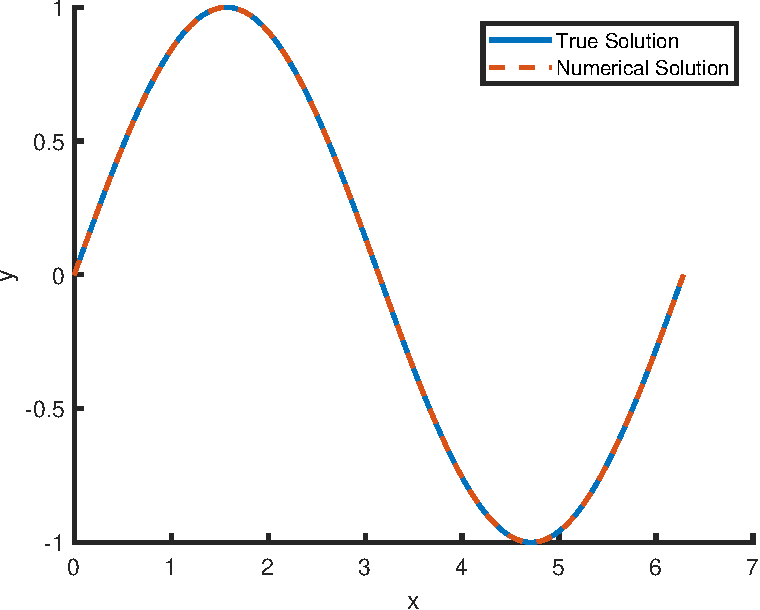
\includegraphics[width=\linewidth]{images/cellAveragecontinue.pdf}
            \caption{smooth}
        \end{minipage}
        \hspace{1cm}
        \begin{minipage}{0.35\linewidth}
            \centering
            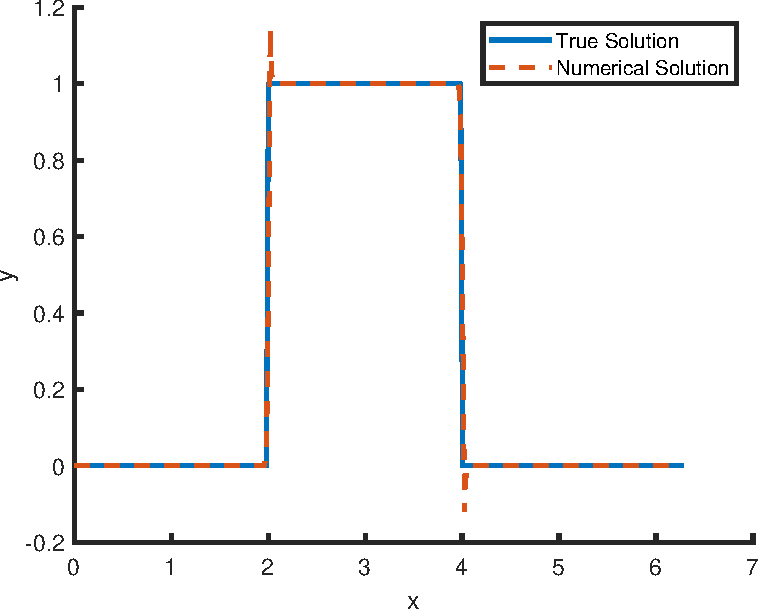
\includegraphics[width=\linewidth]{images/cellAverageDiscontinue.pdf}
            \caption{non-smooth}
        \end{minipage}

        \centering
        \begin{minipage}{0.35\linewidth}
            \centering
            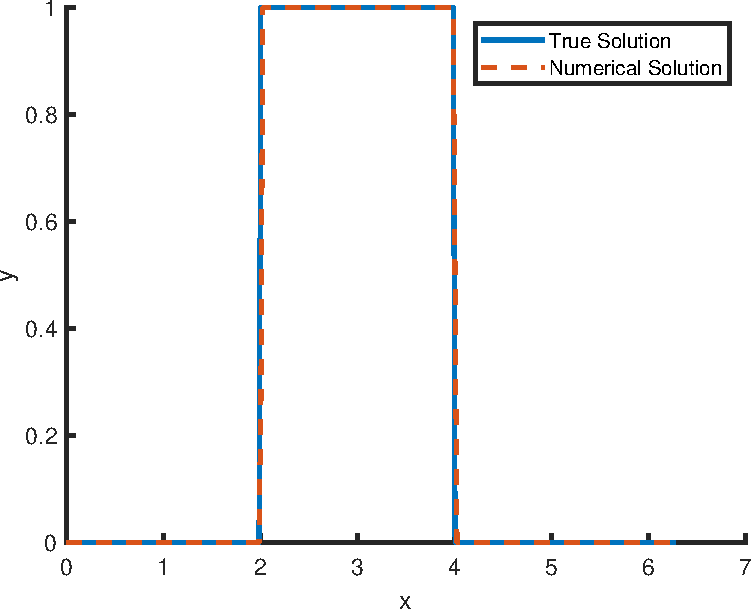
\includegraphics[width=\linewidth]{images/ENODiscontinue.pdf}
            \caption{ENO}
        \end{minipage}
        \hspace{1cm}
        \begin{minipage}{0.35\linewidth}
            \centering
            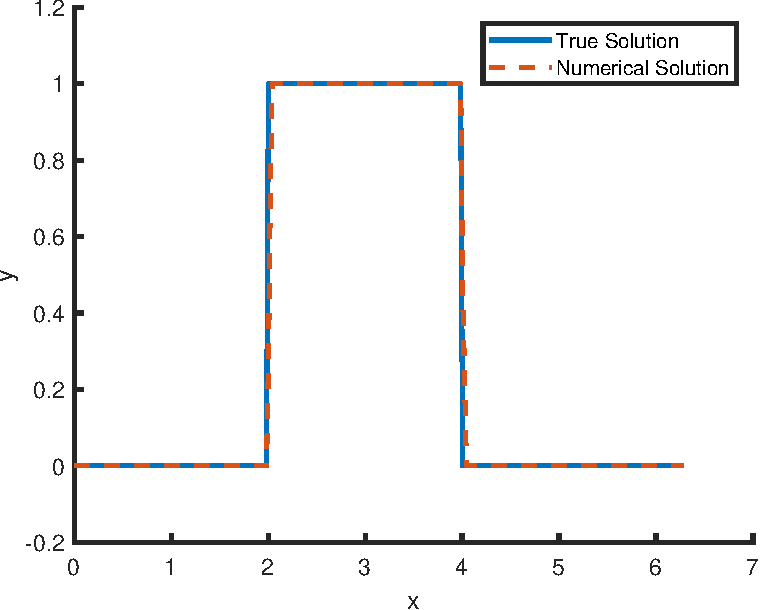
\includegraphics[width=\linewidth]{images/WENODiscontinue.pdf}
            \caption{WENO}
        \end{minipage}

    \end{figure}
\end{frame}
\begin{frame}
    \frametitle{鸣谢}
    \Huge
    \begin{center}
        Thanks
    \end{center}
\end{frame}
\end{document}
